% Circumscribed Parallelepiped
% Author: Axel Pavillet
\documentclass[tikz,border=10pt]{standalone}
%%%<
\usepackage{verbatim}
\usepackage{amsmath, amssymb}
\usepackage{stmaryrd}
\usepackage{graphicx, subfigure}
\usepackage{color}
\usepackage[all]{xy}
\usepackage{extarrows}
\usepackage{proof}
\usepackage{hyperref}
\usepackage{wrapfig}
\usepackage{multirow}

\begin{document}
	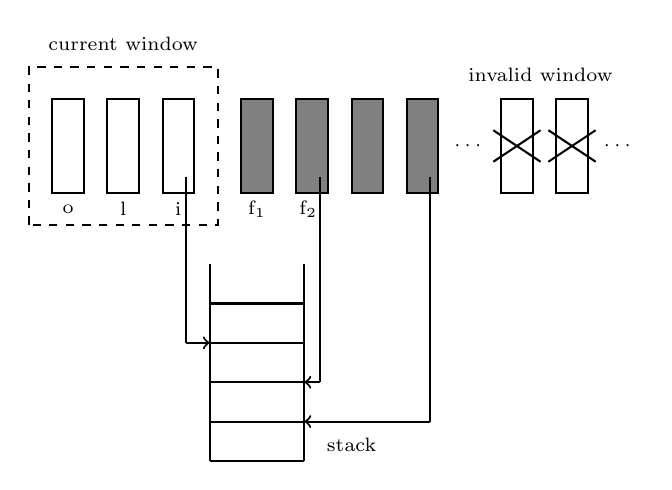
\begin{tikzpicture}[font=\scriptsize, line width=0.75pt]
		\draw[-, dashed] (-0.1,3) rectangle (2.3,5);
        \draw[-] (0.2, 3.4) rectangle (0.6, 4.6);
        \node(o) at (0.4, 3.2) {o};
        \draw[-] (0.9, 3.4) rectangle (1.3, 4.6);
        \node(l) at (1.1, 3.2) {l};
        \draw[-] (1.6, 3.4) rectangle (2, 4.6);
        \node(i) at (1.8, 3.2) {i};
        
        \node(S1) at (1.1, 5.3) {current window};
        
        \filldraw[gray] (2.6, 3.4) rectangle (3, 4.6);
        \draw[-] (2.6, 3.4) rectangle (3, 4.6);
        \node(fm1) at (2.8, 3.2) {$\text{f}_1$};
        \filldraw[gray] (3.3, 3.4) rectangle (3.7, 4.6);
        \draw[-] (3.3, 3.4) rectangle (3.7, 4.6);
        \node(fm2) at (3.45, 3.2) {$\text{f}_2$};
        \filldraw[gray] (4, 3.4) rectangle (4.4, 4.6);
        \draw[-] (4, 3.4) rectangle (4.4, 4.6);
        \filldraw[gray] (4.7, 3.4) rectangle (5.1, 4.6);
        \draw[-] (4.7, 3.4) rectangle (5.1, 4.6);
        
        \node(dot) at (5.5, 4) {$\cdots$};
        
        \draw[-] (5.9, 3.4) rectangle (6.3, 4.6);
        \draw[-] (6.6, 3.4) rectangle (7, 4.6);
        \node(S2) at (6.4, 4.9) {invalid window};
        \draw[-] (5.8, 3.8) to (6.4, 4.2);
        \draw[-] (5.8, 4.2) to (6.4, 3.8);
        \draw[-] (6.5, 3.8) to (7.1, 4.2);
        \draw[-] (6.5, 4.2) to (7.1, 3.8);
        
        \node(dot1) at (7.4, 4) {$\cdots$};
        
        \draw[-] (2.2, 2.5) to (2.2, 0);
        \draw[-] (2.2, 0) to (3.4, 0);
        \draw[-] (3.4, 0) to (3.4, 2.5);
        
        \draw[-] (2.2, 0.5) to (3.4, 0.5);
        \draw[-] (2.2, 1) to (3.4, 1);
        \draw[-] (2.2, 1.5) to (3.4, 1.5);
        \draw[-] (2.2, 2) to (3.4, 2);
        
        \draw[-] (1.9, 3.6) to (1.9, 1.5);
        \draw[->] (1.9, 1.5) to (2.2, 1.5);
        
        \draw[-] (3.6, 3.6) to (3.6, 1);
        \draw[->] (3.6, 1) to (3.4, 1);
        
        \draw[-] (5, 3.6) to (5, 0.5);
        \draw[->] (5, 0.5) to (3.4, 0.5);
        
        \node(st) at (4, 0.2) {stack};
	\end{tikzpicture}
\end{document}
